\section{Asymmetric Numeral System}

% Add outline page for Introduction section
\begin{frame}{Outline}
    \tableofcontents[
        currentsection, 
        sectionstyle=show/hide, 
        subsectionstyle=show/show/hide, 
        subsubsectionstyle=show/show/hide]
\end{frame}

\subsection{Motivation}
    \begin{frame}[fragile]{Motivation}
        ANS combines the compression ratio of \href{https://en.wikipedia.org/wiki/Arithmetic_coding}{arithmetic coding} (which uses a nearly accurate \href{https://en.wikipedia.org/wiki/Probability_distribution}{probability distribution}), with a processing cost similar to that of \href{https://en.wikipedia.org/wiki/Huffman_coding}{Huffman coding} \refer{4}.
    \end{frame}

\subsection{Key Concepts}
    \begin{frame}[fragile]{Key Concepts}
        \begin{itemize}
            \item<1-> \textbf{Symbol spread function} $\rightarrow$ \textcolor{blue}{"Numeral System"}, e.g. standard binary system 
            \item<2-> \textbf{Representation of information}, e.g. standard decimal system \\
            represents an entire message as a single number
            \item<3-> \textbf{Symmetric or \textcolor{blue}{"Asymmetric"}}
        \end{itemize}
    \end{frame}

\subsubsection{Symbol spread function}
    \begin{frame}[fragile]{Symbol spread function}
        \begin{itemize}
            \item<1-> the function that determines the split of the $\mathbb{N}$ subsets corresponding to different symbols \refer{3}
            \item<2-> $\bar{\mathit{s}}: \mathbb{N} \rightarrow \mathcal{A}, \bar{\mathit{s}}(\mathit{x}) = \text{mod}\mathit{(x,b) = s}$
            \item<3-> In the standard binary system example: $\bar{\mathit{s}}(x) = \text{mod}(\mathit{x},2)$ \\ i.e. splits natural numbers into subsets of even/odd numbers \refer{3}
        \end{itemize}
    \end{frame}

    \begin{frame}[fragile]{Symbol spread function (Exa. 1)}
        $\mathit{S}=\{0,1\}$
        \begin{center}
            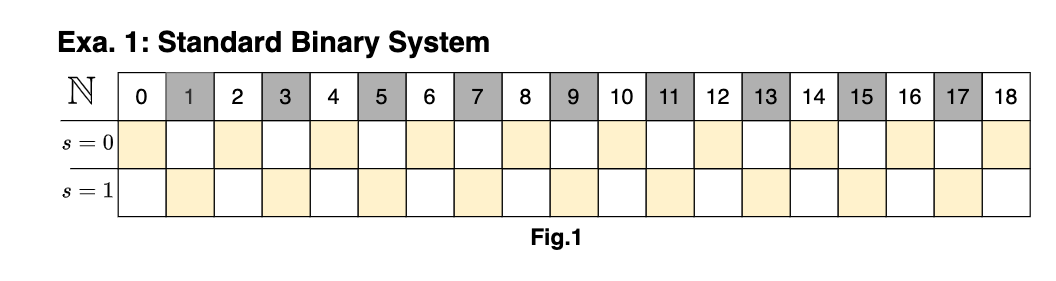
\includegraphics[width=1\textwidth]{../24ws_ANS.assets/fig1.png}
        \end{center}
    \end{frame}

    \begin{frame}[fragile]{Symbol spread function (Exa. 2)}
        $\mathit{S}=\{0,1,2,3,4,5,6,7,8,9\}$
        \begin{center}
            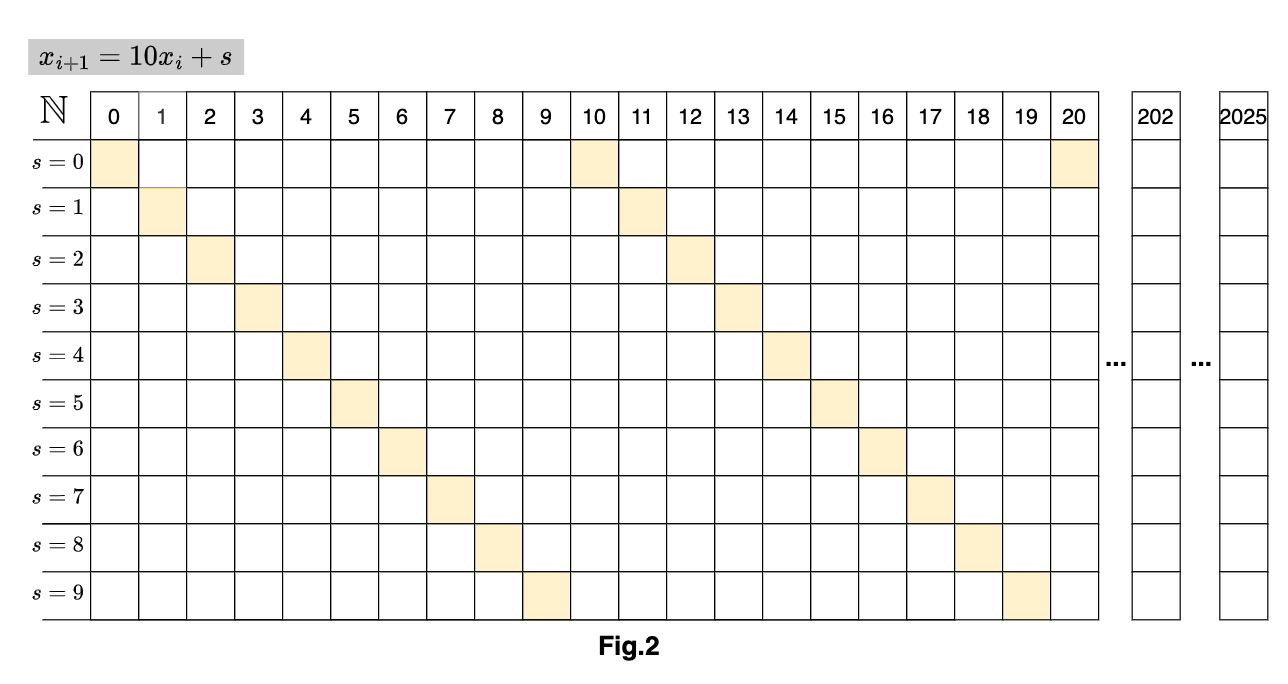
\includegraphics[width=1\textwidth]{../24ws_ANS.assets/fig2.png}
        \end{center}
    \end{frame}

\subsubsection{Representation of information}    
    \begin{frame}[fragile]{Representation of information (Exa. 2)}
        \begin{itemize}
            \item<1-> a finite sequence of symbols/digits: $$\mathcal{A}=\{0,1,2,3,4,5,6,7,8,9\}$$
            \item<2-> the sequence of symbols/digits to be encoded: $$\mathit{S}_{in}=(2,0,2,5)$$
            \item<3-> \textcolor{red}{How can we represent this sequence as a single number?} \\
            The easiest way is to concatenate the symbols/digits: $$\mathit{x}_{out} = 2025$$
        \end{itemize}
    \end{frame}

    \begin{frame}[fragile]{Representation of Information (Exa. 2)}
        \begin{itemize}
            \item<1-> encoding the sequence of digits (2,0,2,5,1,8)
            \[
            \begin{aligned}
                \mathit{x}_{\text{init}} &= 0 \\
                \mathit{x}_1 &= \mathit{x}_{\text{init}} \times 10 + 2 = 2 \\
                \mathit{x}_2 &= \mathit{x}_1 \times 10 + 0 = 20 \\
                \mathit{x}_3 &= \mathit{x}_2 \times 10 + 2 = 202 \\
                \mathit{x}_{\text{out}} &= \mathit{x}_3 \times 10 + 5 = 2025
            \end{aligned}
            \]
        \end{itemize}
    \end{frame}

    \begin{frame}[fragile]{Representation of Information (Exa. 2)}
        \begin{itemize}
            \item<1-> \textcolor{red}{What is the encoding function?}
            \item<2-> Encoding function
            $$\mathit{x_{i+1} = x_i} \times 10 + \mathit{s_i}$$
            \item<3-> $\mathit{x'}$ is the $\mathit{x}$ -th appearance of symbol $\mathit{s}$
            $$\mathit{x'} = \textcolor{orange}{\mathit{C(s, x)= x} \cdot 10 + \mathit{s}} $$
        \end{itemize}
    \end{frame}

    \begin{frame}[fragile]{Representation of Information (Exa. 2)}
        \begin{center}
            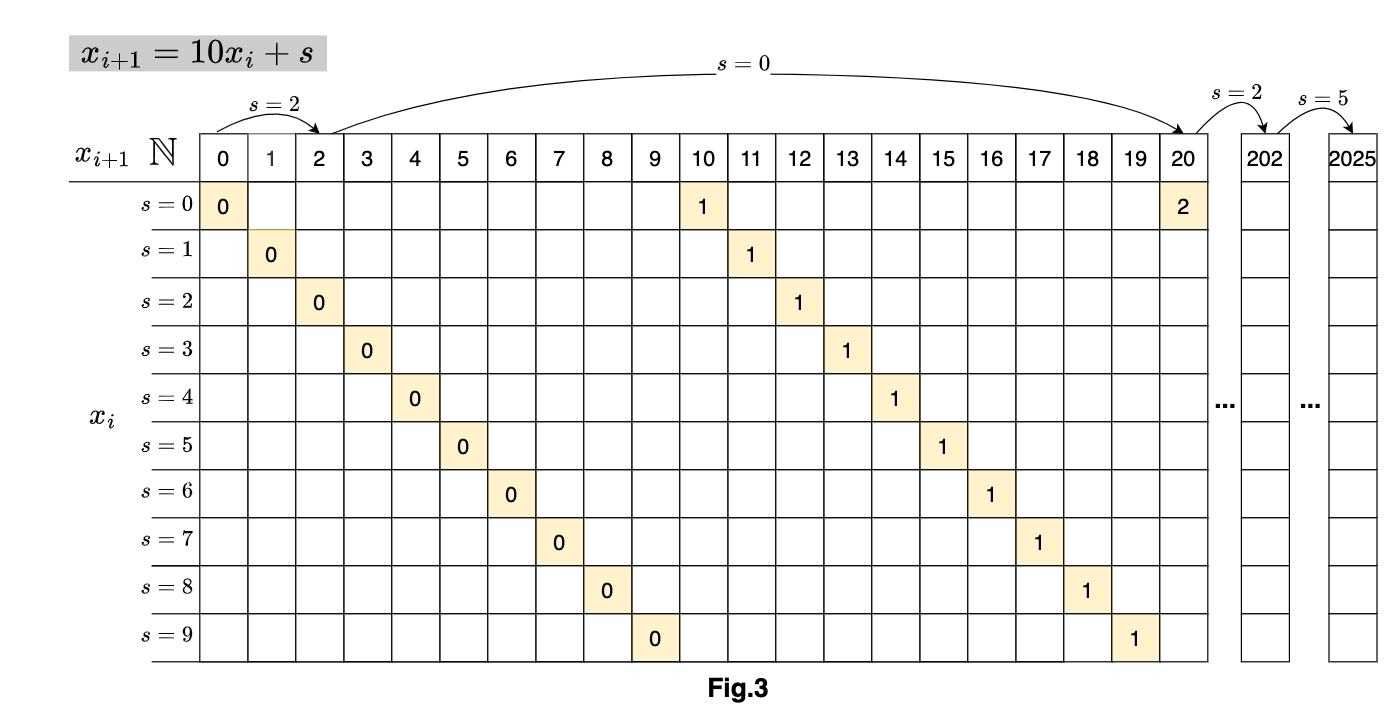
\includegraphics[width=0.85\textwidth]{../24ws_ANS.assets/fig3.png}    
        \end{center}
    \end{frame}

    \begin{frame}[fragile]{Representation of Information (Exa. 1)}
        \begin{center}
            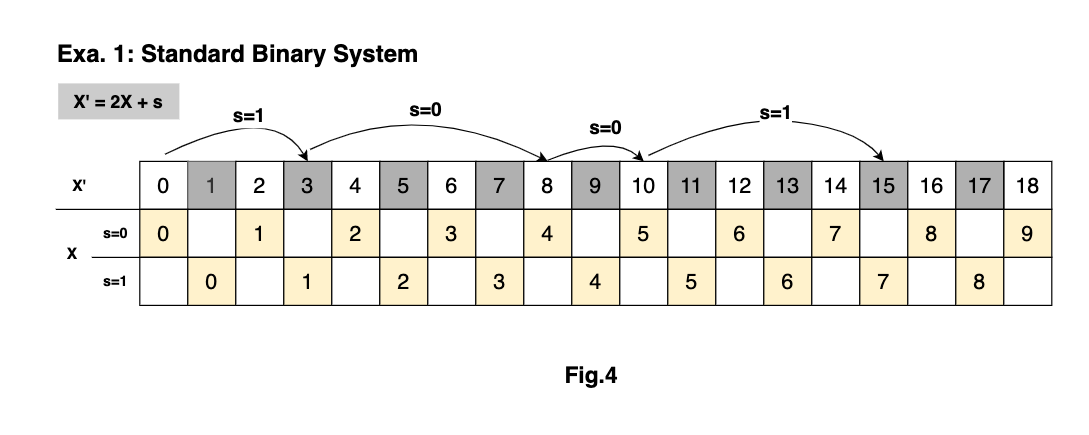
\includegraphics[width=0.95\textwidth]{../24ws_ANS.assets/fig4.png}    
        \end{center}
    \end{frame}

    \begin{frame}[fragile]{}
        \begin{center}
            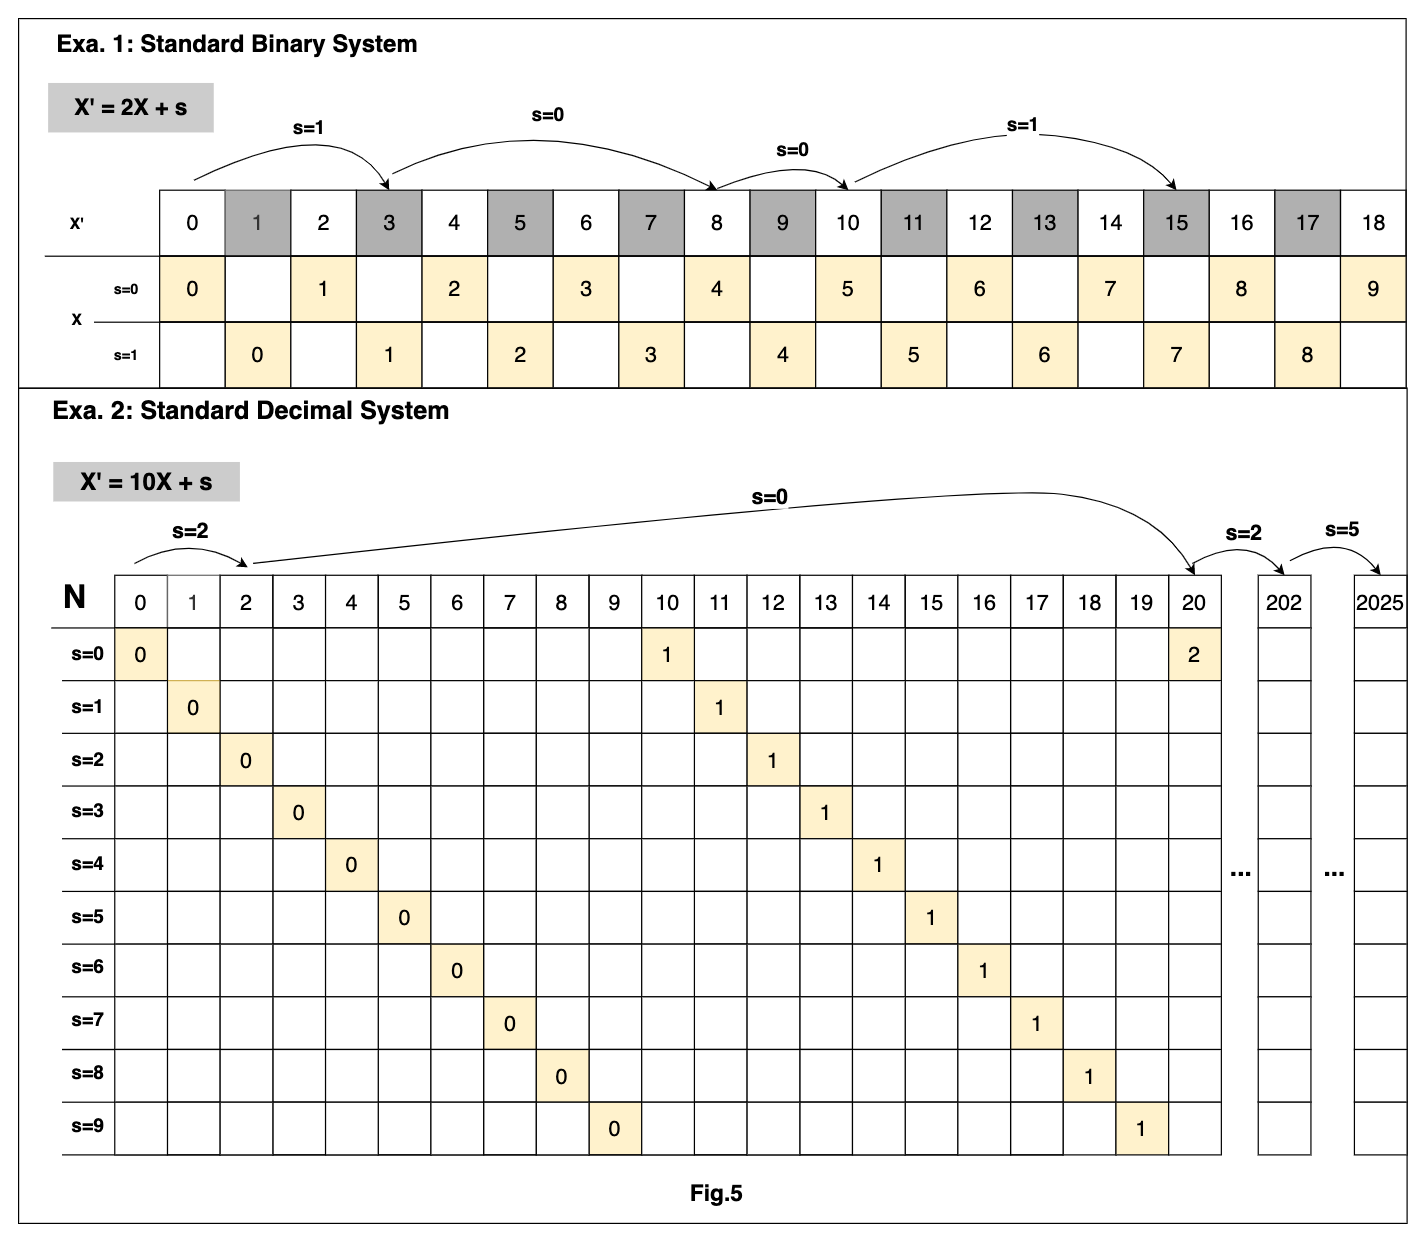
\includegraphics[width=0.7\textwidth]{../24ws_ANS.assets/fig5.png}  
        \end{center}
    \end{frame}

\subsubsection{Symmetric or Asymmetric}
    \begin{frame}[fragile]{}
        \begin{center}
            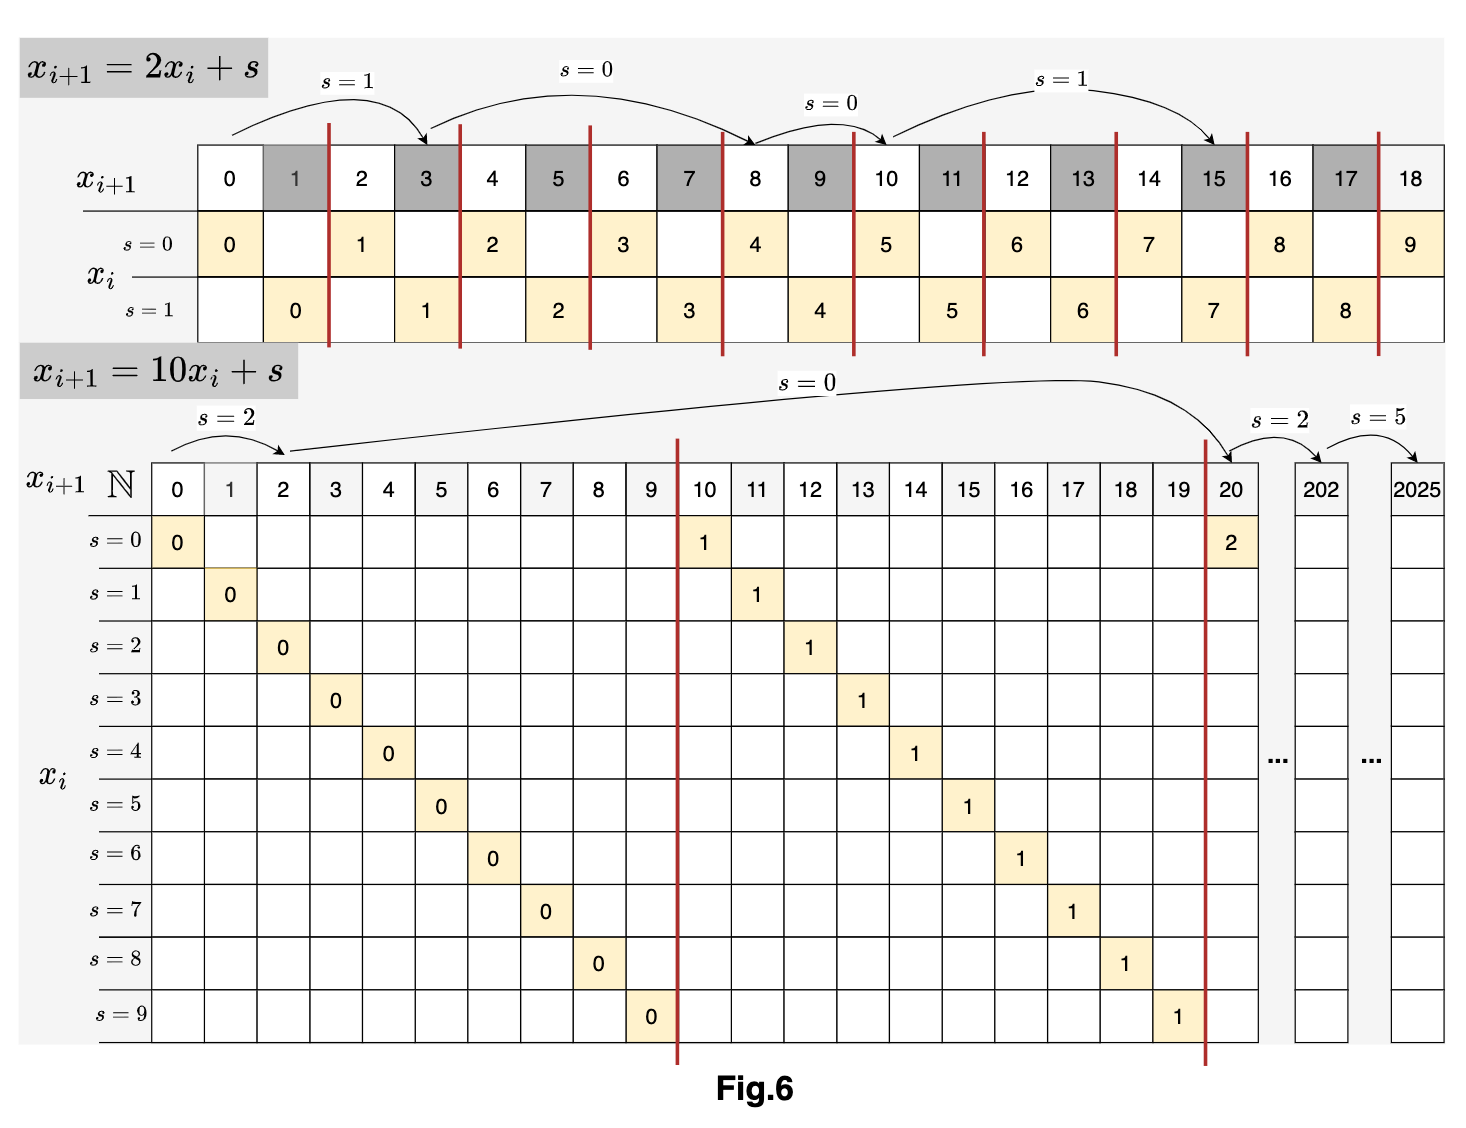
\includegraphics[width=0.7\textwidth]{../24ws_ANS.assets/fig6.png}  
        \end{center}
    \end{frame}

    \begin{frame}[fragile]{Exa. 3: Asymmetric Binary System}
        \begin{itemize}
            \item<1-> Let $\mathcal{A} = \{0,1\}$
            \item<1-> $\mathit{Pr}(0) = 1/4, \mathit{Pr}(1)= 3/4$ 
            \item<2-> a cycle of length 4, which contains 1 zero and 3 ones
            \item<3-> $\mathit{x' = C(s,x) \approx x/p_s}$
            % \item $C(0,x)=4x$, $C(1,x)=4\lfloor x/3 \rfloor + mod(x,3) + 1$
        \end{itemize}
    \end{frame}

    \begin{frame}[fragile]{Exa. 3: Asymmetric Binary System}
        \begin{center}
            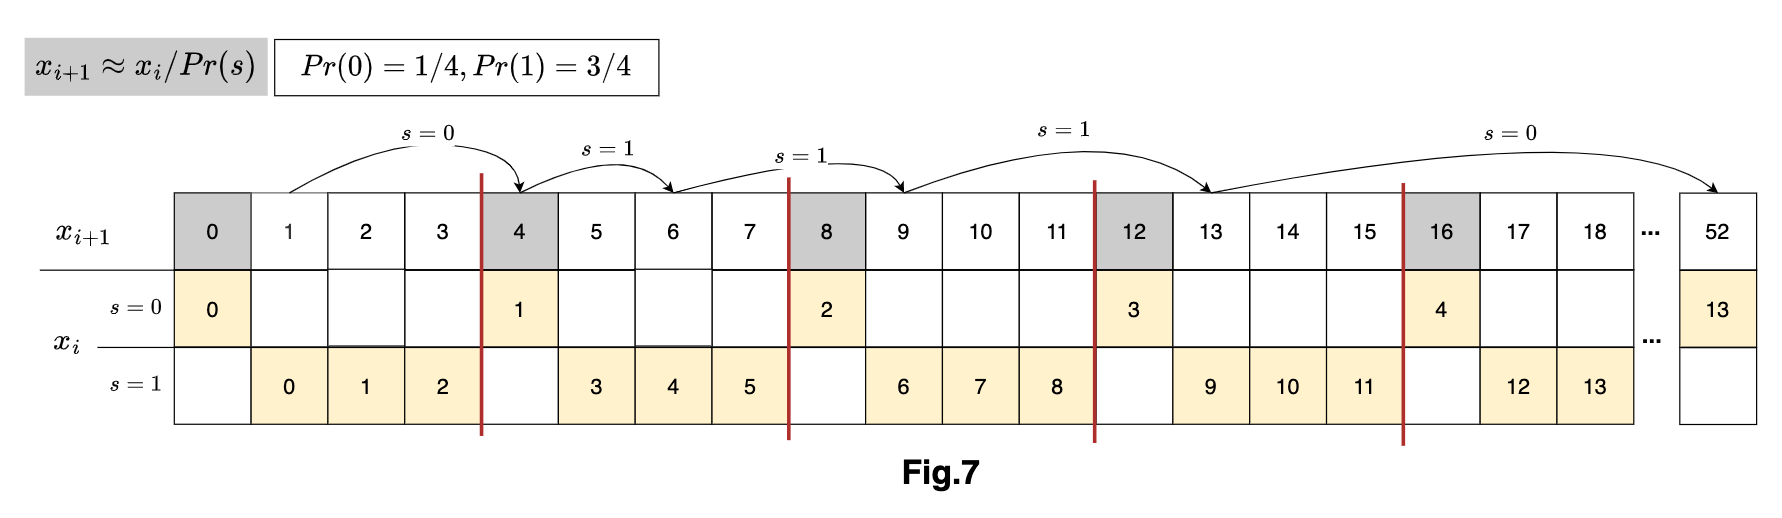
\includegraphics[width=0.9\textwidth]{../24ws_ANS.assets/fig7.png}
        \end{center}
        We refine even/odd number by changing their densities
    \end{frame}

    \begin{frame}[fragile]{Symmetric or Asymmetric}
        \begin{itemize}
            \item Symmetric: uniform distribution
            \item Asymmetric: non-uniform distribution
                \begin{itemize}
                    \item To change the symmetric behavior so that the information added to $\mathit{x}$ by coding a new symbol depends on the probability distribution of the symbols
                    \item $\mathit{log}_2(\mathit{x})$ bits
                    \item A symbol of probability pcarries $\mathit{log}_2(1/\mathit{p})$ bits of information
                    \item How many bits of new information? $\mathit{log}_2\mathit{x} + \mathit{log}_2(1/\mathit{p}) \rightarrow \mathit{log}_2\mathit{x'}$
                    \item $\mathit{log}_2\mathit{x'} = \mathit{log}_2\mathit{x} + \mathit{log}_2(1/\mathit{p}) = \mathit{log}_2(\mathit{x/p}) \Rightarrow \textcolor{orange}{ \mathit{x'} \rightarrow \mathit{x/p}}$
                \end{itemize}
        \end{itemize}
    \end{frame}

\subsection{Performance}
\begin{frame}[fragile]{Performance}
    \begin{itemize}
        \item f
    \end{itemize}
\end{frame}
